\documentclass[11pt,a4paper]{article}

\usepackage{graphicx}
\usepackage{url}
\title{Operating Systems and its Types}
\author{e-Yantra Team}
\date{\today}

\begin{document}
	\maketitle
	\newpage
	\tableofcontents
	\newpage
	\section{Introduction}
	\begin{enumerate}
		\item An operating system (OS) is a software, that manages the computer hardware, and provides common services for execution of various application software.  For hardware functions such as input and output and memory allocation, the operating system acts as an intermediary between application programs and the computer hardware.
		\item An operating system (sometimes abbreviated as "OS") is the program that, after being initially loaded into the computer by a boot program, manages all the other programs in a computer.
		\begin{figure}[h!]
			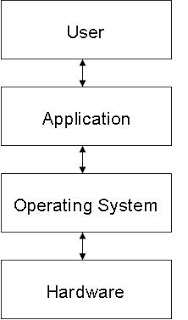
\includegraphics[width=6cm, height=8cm]{os.JPG}
			\centering
		\end{figure} 
	\end{enumerate} 
	\section{Objectives of an OS}
	\begin{itemize}
		\item Convenience: makes computer user friendly.
		\item Efficiency: allows computer to use resources efficiently.
		\item Ability to evolve: constructed in a way to permit effective development, testing and introduction of new functions without interfering with service.
	\end{itemize}
	
	\newpage
	\section{Functions of an OS}
	\begin{enumerate}
		\item Resource Management:  The resource management function of an OS allocates computer resources such as CPU time, main memory, secondary storage, and input and output devices for use.
		\begin{enumerate}
		  \item Process Management:  The operating system is responsible for the following activities in connection with process management:
		  \begin{itemize}
			\item Creating and deleting both user and system processes.
		  	\item Suspending and resuming processes.
		  	\item Providing mechanisms for process synchronization.
		  	\item Providing mechanisms for process communication.
		  	\item Providing mechanisms for deadlock handling.
		  \end{itemize}
		\item Memory Management:  The operating system is responsible for the following activities in connection with memory management:
		\begin{itemize}
			\item Keeping track of which parts of memory are currently being used and by whom.
			\item Deciding which processes and data to move into and out of memory.
			\item Allocating and deallocating memory space as needed.
		\end{itemize}
		\item Storage Management:
		\begin{enumerate}
		\item File – System Management:  The operating system is responsible for the following activities in connection with the file management:
		\begin{itemize}
		\item Creating and deleting files
		\item Creating and deleting directories to organize files.
		\item Supporting primitives for manipulating files and directories.
		\item Mapping files onto secondary storage.
		\item Backing up files on stable (nonvolatile) storage media.	
		\end{itemize}
		\item Mass – Storage Management:  The operating system is responsible for the following activities in connection with disk management:
		\begin{itemize}
		\item Free-space Management
		\item Storage Allocation
		\item Disk Scheduling	
		\end{itemize}
		
		\end{enumerate}
		\item Device Management:  One of the purposes of operating system is to hide the peculiarities of specific hardware devices from the user.
		\end{enumerate}
		\item Data Management:  The data management functions of an OS govern the input and output of the data and their location, storage, and retrieval.
		\item Job Management:  The job management function of an OS prepares, schedules, controls, and monitors jobs submitted for execution to ensure the most efficient processing. A job is a collection of one or more related programs and their data.
		\item Standard means of communication between user and computer:  The OS establishes a standard means of communication between users and their computer systems. It does this by providing a user interface and a standard set of commands that control the hardware. 
		\item In a multitasking operating system where multiple programs can be running at the same time, the operating system determines which applications should run in what order and how much time should be allowed for each application before giving another application a turn.
		\item It manages the sharing of internal memory among multiple applications.
		\item It handles input and output to and from attached hardware devices, such as hard disks, printers, and dial-up ports.
		\item It sends messages to each application or interactive user (or to a system operator) about the status of operation and any errors that may have occurred .
		\item It can offload the management of what are called batch jobs (for example, printing) so that the initiating application is freed from this work .
		\item On computers that can provide parallel processing, an operating system can manage how to divide the program so that it runs on more than one processor at a time .
		\item Operating systems perform basic tasks, such as recognizing input from the keyboard, sending output to the display screen, keeping track of files and directories on the disk, and controlling peripheral devices such as disk drives and printers .
		\item The operating system is also responsible for security, ensuring that unauthorized users do not access the system .
	\end{enumerate}
	
	\section{Types of Operating Systems}
	\begin{enumerate}
	\item Batch Operating System:  Batch operating system is the operating system which analyzes your input and groups them into batches i.e. data in each batch is of similar characteristics. And then it performs operation on each individual batch.
	\item Real-time:  A real-time operating system is a multitasking operating system that aims at executing real-time applications. Real-time operating systems often use specialized scheduling algorithms so that they can achieve a deterministic nature of behavior. The main object of real-time operating systems is their quick and predictable response to events. They either have an event-driven or a time-sharing design. An event-driven system switches between tasks based on their priorities while time-sharing operating systems switch tasks based on clock interrupts.
	\begin{itemize}
		\item Hard real-time system:  It has the most stringent requirements, guaranteeing that real-time tasks be completed within their deadlines. Safety-critical systems are typically hard real-time systems.
		\item Soft real-time system:  It is less restrictive, simply providing that a critical real-time task will receive priority over other tasks and that it will retain that priority until it completes. Many commercial operating systems – as well as Linux – provide soft real-time support.
	\end{itemize}
	\item Multi-user vs. Single-user:  A multi-user operating system allows multiple users to access a computer system concurrently. Time-sharing system can be classified as multi-user systems as they enable a multiple user access to a computer through the sharing of time. Single-user operating systems, as opposed to a multi-user operating system, are usable by a single user at a time. Being able to have multiple accounts on a Windows operating system does not make it a multi-user system. Rather, only the network administrator is the real user. But for a Unix-like operating system, it is possible for two users to login at a time and this capability of the OS makes it a multi-user operating system.
	\item Multi-tasking vs. Single-tasking:  When a single program is allowed to run at a time, the system is grouped under a single-tasking system, while in case the operating system allows the execution of multiple tasks at one time, it is classified as a multi-tasking operating system. Multi-tasking can be of two types namely, pre-emptive or co-operative. In pre-emptive multitasking, the operating system slices the CPU time and dedicates one slot to each of the programs. Unix-like operating systems such as Solaris and Linux support pre-emptive multitasking. Cooperative multitasking is achieved by relying on each process to give time to the other processes in a defined manner. MS Windows prior to Windows 95 used to support cooperative multitasking.
	\item Single-processor Systems:  On a single-processor system, there is one main CPU capable of executing a general-purpose instruction set, including instructions from user processes.
	\item Multi-processor Systems:  A multiprocessing operating system allows a program to run on more than one central processing unit (CPU) at a time. This can come in very handy in some work environments, at schools, and even for some home-computing situations.
	\begin{itemize}
	\item Asymmetric multiprocessing:  In this each processor is assigned a specific task. A master processor controls the system; the other processors either look to the master for instruction or have predefined tasks. This scheme defines a master-slave relationship. The master processor schedules and allocates work to the slave processors.
	\item Symmetric multiprocessing (SMP):  In this each processor performs all tasks within the operating system. SMP means that all processors are peers; no master-slave relationship exists between processors.
	\end{itemize}
	\item Distributed:  A distributed operating system manages a group of independent computers and makes them appear to be a single computer. The development of networked computers that could be linked and communicate with each other, gave rise to distributed computing. Distributed computations are carried out on more than one machine. When computers in a group work in cooperation, they make a distributed system.
	\item Embedded: Embedded operating systems are designed to be used in embedded computer systems. They are designed to operate on small machines like PDAs with less autonomy. They are able to operate with a limited number of resources. They are very compact and extremely efficient by design. Windows CE and Minix 3 are some examples of embedded operating systems.
	\end{enumerate}
	
	\newpage
	\section{Examples of Operating System}
	\begin{itemize}
		\item DOS (Disk Operating System) was the first widely-installed operating system for personal computers. It is a master control program that is automatically run when you start your PC. DOS stays in the computer all the time letting you run a program and manage files. It is a single-user operating system from Microsoft for the PC. It was the first OS for the PC and is the underlying control program for Windows 3.1, 95, 98 and ME. Windows NT, 2000 and XP emulate DOS in order to support existing DOS applications. To use DOS, you must know where your programs and data are stored and how to talk to DOS.
			\begin{figure}[h!]
				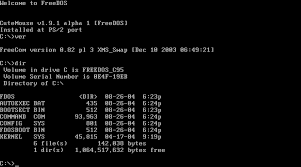
\includegraphics{dos.png}
				\centering
			\end{figure} 
		\item UNIX operating systems are used in widely-sold workstation products from Sun Microsystems, Silicon Graphics, IBM, and a number of other companies. The UNIX environment and the client/server program model were important elements in the development of the Internet and the reshaping of computing as centered in networks rather than in individual computers. Linux, a UNIX derivative available in both "free software" and commercial versions, is increasing in popularity as an alternative to proprietary operating systems.UNIX is written in C. Both UNIX and C were developed by AT\&T and freely distributed to government and academic institutions, causing it to be ported to a wider variety of machine families than any other operating system. As a result, UNIX became synonymous with "open systems."The Unix-like family is a diverse group of operating systems, with several major sub-categories including System V, BSD, and Linux.
		\newpage
			\begin{figure}[h!]
				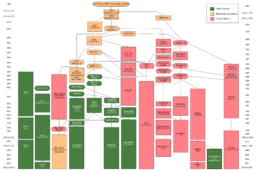
\includegraphics[width=10cm, height=8cm]{Unix.png}
				\centering
			\end{figure} 
		\item A subgroup of the Unix family is the Berkeley Software Distribution family, which includes FreeBSD, NetBSD, and OpenBSD. These operating systems are most commonly found on webservers, although they can also function as a personal computer OS. The Internet owes much of its existence to BSD, as many of the protocols now commonly used by computers to connect, send and receive data over a network were widely implemented and refined in BSD. The World Wide Web was also first demonstrated on a number of computers running an OS based on BSD called NextStep.
		
		\item The Macintosh (often called "the Mac"), introduced in 1984 by Apple Computer, was the first widely-sold personal computer with a graphical user interface (GUI). The Mac was designed to provide users with a natural, intuitively understandable, and, in general, "user-friendly" computer interface. This includes the mouse, the use of icons or small visual images to represent objects or actions, the point-and-click and click-and-drag actions, and a number of window operation ideas. Microsoft was successful in adapting user interface concepts first made popular by the Mac in its first Windows operating system. The primary disadvantage of the Mac is that there are fewer Mac applications on the market than for Windows. However, all the fundamental applications are available, and the Macintosh is a perfectly useful machine for almost everybody.
			\begin{figure}
				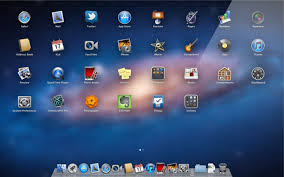
\includegraphics{mac.jpg}
				\centering
			\end{figure} 
		\newpage
		\item Windows is a personal computer operating system from Microsoft that, together with some commonly used business applications such as Microsoft Word and Excel, has become a de facto "standard" for individual users in most corporations as well as in most homes. Windows contains built-in networking, which allows users to share files and applications with each other if their PCs are connected to a network. In large enterprises, Windows clients are often connected to a network of UNIX and NetWare servers.
			\begin{figure}[h!]
				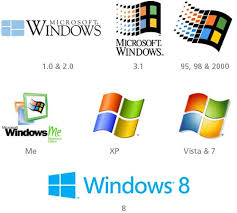
\includegraphics{windows.jpg}
				\centering
			\end{figure}
		\newpage 
		\item The Linux open source operating system, or Linux OS, is a freely distributable, cross-platform operating system based on Unix that can be installed on PCs, laptops, netbooks, mobile and tablet devices, video game consoles, servers, supercomputers and more.The Linux OS is frequently packaged as a Linux distribution for both desktop and server use, and includes the Linux kernel (the core of the operating system) as well as supporting tools and libraries. Popular Linux OS distributions include Debian, Ubuntu, Fedora, Red Hat and openSUSE.
		\begin{figure}[h!]
			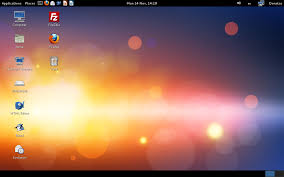
\includegraphics{linux.jpg}
			\centering
		\end{figure} 
		\item There have been many operating systems that were significant in their day but are no longer so, such as AmigaOS; OS/2 from IBM and Microsoft; Mac OS, the non-Unix precursor to Apple's Mac OS X; BeOS; XTS-300; RISC OS; MorphOS; Haiku; BareMetal and FreeMint. Some are still used in niche markets and continue to be developed as minority platforms for enthusiast communities and specialist applications. OpenVMS, formerly from DEC, is still under active development by Hewlett-Packard. Yet other operating systems are used almost exclusively in academia, for operating systems education or to do research on operating system concepts. A typical example of a system that fulfills both roles is MINIX, while for example Singularity is used purely for research.
	\end{itemize}
	
	\newpage
	\section{Raspbian Operating System}
	Debian is a Unix-like computer operating system and a Linux distribution that is composed entirely of free and open-source software, most of which is under the GNU General Public License, and packaged by a group of individuals known as the Debian project. Currently, the Debian project offers three branches named "stable", "testing" and "unstable".Debian has access to online repositories that contain over 43,000 software packages.Debian officially contains only free software, but non-free software can be downloaded from the Debian repositories and installed.Debian includes popular free programs such as LibreOffice, Iceweasel (FireFox) web browser, Evolution mail, K3b disc burner, VLC media player, GIMP image editor and Evince document viewer.Debian is a popular choice for web servers.
		\begin{figure}[h!]
			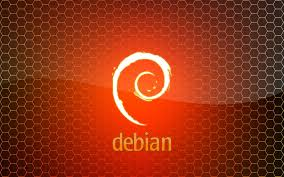
\includegraphics[width=7cm]{d.jpg}
			\centering
		\end{figure} 
		
	Raspbian is a free operating system based on Debian optimized for the Raspberry Pi hardware. An operating system is the set of basic programs and utilities that make your Raspberry Pi run.based on the ARM hard-float (armhf) Debian 7 'Wheezy' architecture port originally designed for ARMv7 and later processors (with Jazelle RCT/ThumbEE, VFPv3, and NEON SIMD extensions), compiled for the more limited ARMv6 instruction set of the Raspberry Pi.
	\begin{figure}[h!]
		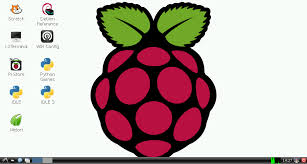
\includegraphics[width=7cm]{Raspbian.jpg}
		\centering
	\end{figure} 
	 
	 \newpage
	\section{References}
	\begin{itemize}
		\item \url{http://www.webopedia.com/TERM/L/linux_os.html}
		\item \url{http://homepages.uel.ac.uk/u0114353/sec4.html}
		\item \url{http://operatingsystemfundas.blogspot.in/2012/05/post1.html}
		\item \url{http://en.wikipedia.org/wiki/Debian}
		\item \url{http://en.wikipedia.org/wiki/Raspberry_Pi}
		\item \url{https://www.raspberrypi.org}
		\item \url{http://en.wikipedia.org/wiki/Operating_system}
		\item \url{https://www.google.co.in}
	\end{itemize}
	
\end{document}



